\documentclass[]{article}

\usepackage{graphicx}
\usepackage{caption}
\usepackage{subfig}
\usepackage{listings}

%opening
\title{Systems Biology Project 3}
\author{Mathias D. Kallick}

\begin{document}
	
	\maketitle
	
	\section{Genetic Algorithms}
	Genetic algorithms are a computational technique used in Systems Biology to fit parameters to a model. Instead of relying on manually selected parameters, or something like a grid-search, where sets of parameters evenly covering the parameter space are tested, genetic algorithms rely on a more biologically inspired algorithm to speed up parameter fitting. In a genetic algorithm, you start by generating a set of parents, which are simply parameter sets that we can run the model with. We test each parameter set against a cost function, and in doing so determine how "good" that parameter set is. In a genetic algorithm, the quality of the parent determines the likelihood that it will be used as a parent for the next generation, but even the worst parent can be selected to generate a child. For the next generation, you pick parents according to a selection method, then you use those to generate the children (in our case, this means randomly mixing the parameters), and then you perturb each parameter a little bit to vary the data. You then do this for multiple generations, and because you make better parents more likely to be chosen to create children, each generation gets progressively better. In this way, a genetic algorithm can generate a very good parameter set without requiring exhaustive searching of a parameter space for the best parameters. It is also much less likely than a greedy algorithm to hit a local "best" parameter set that doesn't actually provide relatively good performance compared to the theoretical optimum parameters. \\
	
	\subsection{Cost Function}
	To use genetic algorithms (or an evolutionary strategy), there must be a way to quantify the "goodness" of a parameter set. This is the job of a cost function, which takes the parameters and returns a cost (low for a good fit, high for a bad one). In our case, this involves running the model with that parameter set for $800$ hours with a dt of $.1$ (this is where a lot of the time cost complexity comes in). I then calculate the period and amplitude of the second half of that data (allowing the first half as a startup period where the oscillations stabilize), and check them against the desired period and amplitude. I want a period of $23.6$ hours, and an amplitude that is not lower than $.1$. I use the squared difference between the period and the desired period, divided by the desired period, to calculate my error value for period. I use the natural log of $.001$ over the desired amplitude, multiplied by the actual amplitudes (here I use all of the amplitudes for all of the variables in the model). I then take the exponent of those values, and average them out to get the error value for my amplitude. My total error is simply the sum of those two errors. \\
	
	\subsection{Elite Carryover}
	For genetic algorithms, it is not uncommon for the best member of the next generation to actually be worse than the best member of the current generation - perhaps the parents happened to be randomly chosen badly, or perhaps the mixing of the best parents created a worse solution. To deal with this, we can pick some number of "elite" members of the current generation (the best members according to the cost function). Then we simply place those "elites" into the next generation without changing them at all - this means that we cannot possibly get worse from one generation to the next, because we retain the best value(s) from the previous generation. \\
	
	\subsection{Selection Methods}
	Selection methods are an important part of any genetic algorithm. Essentially, they represent the way that parents are selected for each child in the next generation. In my code, we first pick all of the parents for the next generation (some parents can be used multiple times, and it is also possible that a child has two of the same parent), and then generate the children with those parents. \\
	
	\subsubsection{Tournament Selection}
	Tournament selection is a way of picking lots of "local best" parents, which decreases the likelihood of a single "best" parameter set being beelined towards. Instead it provides some diversity in the resulting parameter sets. The idea behind tournament selection is to pick groups of children from the previous generation and find the best performer among each group (which is a small subset of the total child population). The best performers are then used as the parents of the next generation. The other advantage to tournament selection is that you never have to sort the list entirely. Thus, you get a better time complexity, because you only have to sort small subsets of the list, and sorting a list has a high time complexity. \\
	
	I used $40$ parents and $40$ children over $8$ generations with one elite per generation, and a mutation factor of $.005$. I used a tournament size of $4$. \\
	
	In my test, tournament selection was capable of reducing cost by approximately $-2.19E-05$ per generation (starting at a cost of $1.54E-04$, and ending at $1.28E-06$, over $8$ generations). I noticed that tournament selection tended to find a good cost pretty quickly, but then got stuck on it for a while, staying constant for a few generations before finding a better one. \\
	
	I also found that each generation took about 15 seconds to run, on my machine. \\
	
	See Figure \ref{fig:ts1.1} for the plot generated using the parameters found with tournament selection.
	
	\begin{figure}[!htbp]
		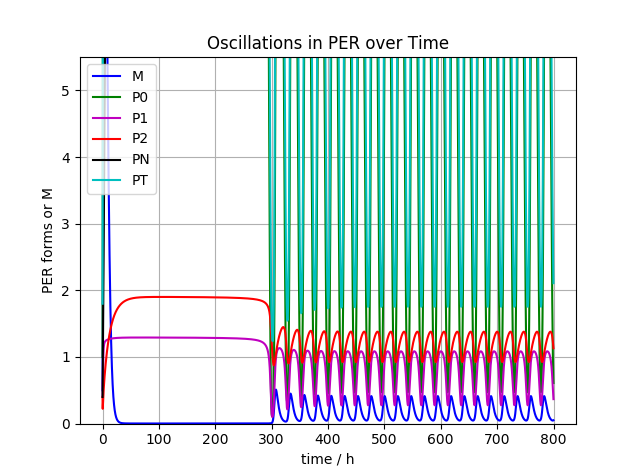
\includegraphics[width=\linewidth]{{"../plots/tourney_1.1"}.png}
		\caption{A simulation of the Goldbeter fly model using parameters (found with tournament selection): $n$ : $8.91$, $K_1$ : $8.67$, $K_2$ : $6.53$, $K_3$ : $1.00$, $K_4$ : $6.21$, $K_m$ : $7.09$, $K_d$ : $9.15$, $K_I$ : $5.48$, $V_1$ : $9.35$, $V_2$ : $6.43$, $V_3$ : $6.94$, $V_4$ : $1.72$, $v_m$ : $5.52$, $v_d$ : $6.22$, $v_s$ : $2.06$, $k_1$ : $8.55$, $k_2$ : $7.74$, $k_s$ : $3.36$}
		\label{fig:ts1.1}
	\end{figure}
	\subsubsection{Linear Ranking Selection}
	Linear Ranking Selection is designed to allow any parents to be selected for the next generation, while making it more likely for the best ones to be chosen. The general idea is to sort the parents by quality, and then use a linear function to give each one a probability of being chosen - that makes the best one most likely to be chosen, but doesn't make it so unlikely to pick the worst parents that they never get chosen. This provides good diversity while also allowing for consistent improvement across generations. This selection method has one distinct disadvantage over tournament selection, which is that it requires a full sort of the parents, which increases the amount of time it needs to run. \\
	
	I used $40$ parents and $40$ children over $8$ generations with one elite per generation, and a mutation factor of $.005$. I used an $\eta^-$ (which determines the slope of the probability line) of $.1$. \\
	
	In my test, linear ranking selection was capable of reducing cost by approximately $-4.73E-05$ per generation (starting at a cost of $3.82E-04$, and ending at $5.11E-05$, over $8$ generations). I noticed that linear selection was far more likely to get stuck on a particular parameter set - it would often stay on the same one for all $8$ generations, and most commonly only go through $2$ or $3$ sets in all of the generations. \\
	
	I also found that each generation took about 16 seconds to run, on my machine. \\
	
	See Figure \ref{fig:lr1.1} for the plot generated using the parameters found with linear ranking selection.
	
	\begin{figure}[!htbp]
		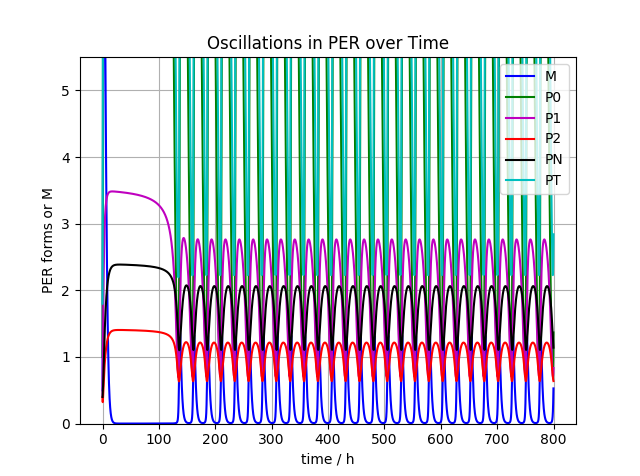
\includegraphics[width=\linewidth]{{"../plots/linear_1.1"}.png}
		\caption{A simulation of the Goldbeter fly model using parameters (found with linear ranking selection): $n$ : $7.79$, $K_1$ : $4.72$, $K_2$ : $4.42$, $K_3$ : $3.23$, $K_4$ : $7.68$, $K_m$ : $9.71$, $K_d$ : $3.14$, $K_I$ : $5.93$, $V_1$ : $9.24$, $V_2$ : $3.68$, $V_3$ : $4.42$, $V_4$ : $4.78$, $v_m$ : $7.60$, $v_d$ : $7.37$, $v_s$ : $9.73$, $k_1$ : $9.93$, $k_2$ : $1.61$, $k_s$ : $5.42$}
		\label{fig:lr1.1}
	\end{figure}

	\subsubsection{Truncation Selection}
	Truncation selection is designed to remove all of the weakest parents from the group (anything below the top fraction of the parents, the size of which is determined by the truncation threshold). Instead of having the chance to pick any of the parents, but being far more likely to pick the better parents, truncation selection works more like an evolutionary strategy. It requires us to sort the entire list of parents (although we could potentially speed this up if our truncation threshold is low enough), and then we simply remove everything below the top fraction of the list (determined by the truncation threshold). We then pick the number of parents that we need for the next generation from that subset of parents (this actually requires that we pick at least one parent more than once, and it is most likely that a lot of them will be picked multiple times). This method removes some of the diversity that we get from the other algorithms, but it does allow us to improve our cost faster if we don't get too greedy (obviously how much those things are true depends on the size of our threshold). In theory, this selection method should be relatively slow because of the full sort for each generation. \\
	
	I used $40$ parents and $40$ children over $8$ generations with one elite per generation, and a mutation factor of $.005$. I used a truncation threshold of $.5$. \\ 
	
	In my test, linear ranking selection was capable of reducing cost by approximately $-1.73E-05$ per generation (starting at a cost of $1.21E-04$, and ending at $3.19E-07$, over $8$ generations). I noticed that truncation selection was also quite likely to get stuck on a particular parameter set - it would often stay on the same one for all $8$ generations, and most commonly only go through $2$ or $3$ sets in all of the generations (just like linear ranking selection). \\
	
	I also found that each generation took about 11 seconds to run, on my machine, which is interesting because in theory they should take longer than the others. \\
	
	See Figure \ref{fig:trunc1.1} for the plot generated using the parameters found with linear ranking selection.
	
	\begin{figure}[!htbp]
		\includegraphics[width=\linewidth]{{"../plots/trunc1.1"}.png}
		\caption{A simulation of the Goldbeter fly model using parameters (found with truncation selection): $n$ : $8.25$, $K_1$ : $2.80$, $K_2$ : $1.47$, $K_3$ : $7.35$, $K_4$ : $5.24$, $K_m$ : $7.66$, $K_d$ : $5.42$, $K_I$ : $7.66$, $V_1$ : $8.73$, $V_2$ : $1.83$, $V_3$ : $9.22$, $V_4$ : $2.12$, $v_m$ : $8.95$, $v_d$ : $8.66$, $v_s$ : $1.62$, $k_1$ : $6.48$, $k_2$ : $4.54$, $k_s$ : $8.22$}
		\label{fig:trunc1.1}
	\end{figure}
		
	\section{Evolutionary Strategy}
	The evolutionary strategy method for parameter fitting is very similar to genetic algorithms, but with a few key differences. When choosing the parents of the next generation, an evolutionary strategy first picks a subset of the available parents - then it picks randomly from that subset for each child. This eliminates the possibility of having all of the parents generate the next generation, unlike a genetic algorithm. Other differences are that we have less parents than children, and we don't use elites at all.
	
	I used $8$ parents and $40$ children over $8$ generations with a mutation factor of $.005$. \\
	
	In my test, my evolutionary strategy was capable of reducing cost by approximately $-5.76E-04$ per generation (starting at a cost of $4.05E-03
	$, and ending at $2.04E-05$, over $8$ generations). The evolutionary strategy was able to reduce cost much more (on average) per generation, but ended within a reasonable margin of the other algorithms, because the cost tended to start out being much higher than the other algorithms. It also had a tendency to occasionally have an increase in cost from one generation to the next (this is possible because it doesn't use elites). \\
	
	I also found that each generation took about 13 seconds to run, on my machine. \\
	
	See Figure \ref{fig:es1.1} for the plot generated using the parameters found using an evolutionary strategy.
	
	\begin{figure}[!htbp]
		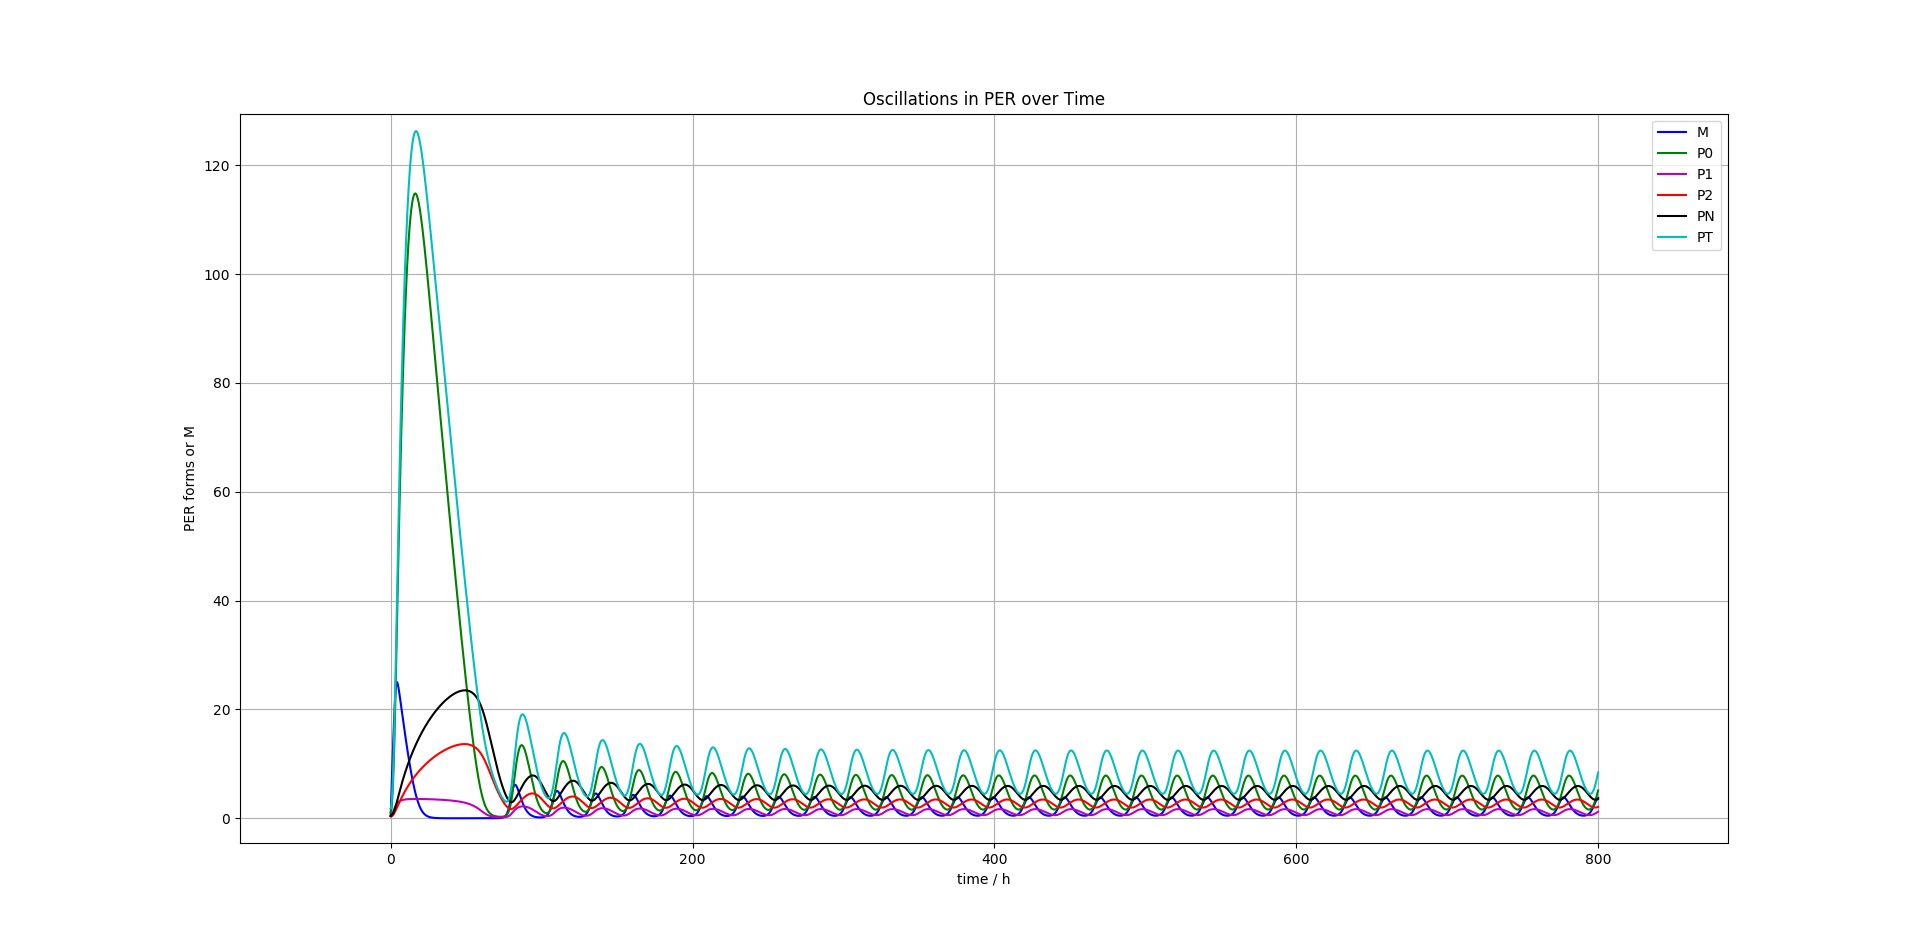
\includegraphics[width=\linewidth]{{"../plots/es_1.1"}.png}
		\caption{A simulation of the Goldbeter fly model using parameters (found using an evolutionary strategy): $n$ : $9.71$, $K_1$ : $10.00$, $K_2$ : $10.00$, $K_3$ : $8.31$, $K_4$ : $9.38$, $K_m$ : $9.06$, $K_d$ : $2.16$, $K_I$ : $1.52$, $V_1$ : $8.26$, $V_2$ : $2.17$, $V_3$ : $4.36$, $V_4$ : $7.82$, $v_m$ : $5.51$, $v_d$ : $5.70$, $v_s$ : $7.34$, $k_1$ : $7.77$, $k_2$ : $1.29$, $k_s$ : $1.11$}
		\label{fig:es1.1}
	\end{figure}
	
	\section{Discussion}
	The results we get here in terms of the quality of each of these algorithms are very interesting. Purely in terms of the cost function, all of these algorithms ended up with roughly equal performance (with the exception of truncation selection, which did quite well). I am quite lenient when I say equal performance because both genetic algorithms and evolutionary strategies are inherently random. In terms of how much the algorithms improved the parameters from one generation to the next, my evolutionary strategy performed the best, but that must be balanced with the fact that it generated a much worse initial cost compared to the others. In terms of time complexity, if we trust the numbers that I measured, truncation selection once again takes the lead. I say if we trust, however, because I ran these at different times, and I don't think that my computer provides even performance over time in that way (mostly because of Windows being written that way, but also because my CPU adapts its clock speed over time based on temperature). \\
	
	If I had to pick one of these algorithms for this model, though, I would pick the evolutionary strategy. This is because it seems to perform at approximately the same level as the other selection algorithms used here, and is about the same speed. However, for this number of generations, the biggest time cost is not actually the cost of running each generation - it is the cost of creating the first parents randomly. This takes a while because we don't want parameter sets that don't generate oscillations, which means that each time we generate one of those, we need to throw it out. Because there are a limited number of sets that will create oscillations, it takes a while to randomly generate one. This favors the evolutionary strategy because it uses substantially less parents than the genetic algorithms. \\
	
	Another thing that is worth noting is that our cost function is very simple - it only cares about period and amplitude. This leads to some strange-looking plots because every other aspect of the model is ignored. Also, because I only run the cost function on the second half of the data, we sometimes get plots that have really strange behavior for the first half but then fall into a really nice oscillation, like in Figure \ref{fig:ts1} (this is also a very good example of oscillations that have a different shape from what we want, but still have the correct period and amplitude). \\

 	\begin{figure}[!htbp]
	 	\includegraphics[width=\linewidth]{{"../plots/tourney_1"}.png}
	 	\caption{A simulation of the Goldbeter fly model using found parameters. This is a good example of what happens when the cost function is very simple.}
	 	\label{fig:ts1}
	 \end{figure}
 
 	To conclude, we will look at an interesting observation that Goldbeter made, which is that when you increase the PER degradation rate ($v_d$), you also increase the maximum amount of PER in the system (i.e. the top of the oscillation). Using a different parameter set I tested this observation, and as can be seen in Figure \ref{fig:vds} and Figure \ref{fig:vds2}, this holds true for multiple parameter sets. I found that increasing the PER degradation rate also increases maximum total PER for two distinct parameter sets that are also distinct from Goldbeter's model. \\
	
	
	\begin{figure}[!htbp]
	 	\includegraphics[width=\linewidth]{{"../plots/vds"}.png}
	 	\caption{Simulations of the Goldbeter fly model using found parameters, with varying values for the parameter $v_d$. This provides support for Goldbeters's claim that increasing $v_d$ also increases maximum total PER. The initial parameters were found with an evolutionary strategy.}
	 	\label{fig:vds}
	\end{figure}
	
	\begin{figure}[!htbp]
		\includegraphics[width=\linewidth]{{"../plots/vds2"}.png}
		\caption{Simulations of the Goldbeter fly model using found parameters, with varying values for the parameter $v_d$. This provides support for Goldbeters's claim that increasing $v_d$ also increases maximum total PER. Notice that some of these values of $v_d$ barely provide good oscillation, but it is still distinctly noticeable that PER levels change. The initial parameters were found with linear ranking selection.}
		\label{fig:vds2}
	\end{figure}
	
\end{document}
